%% Copyright 2007-2020 Elsevier Ltd
%% 
%% This file is part of the 'Elsarticle Bundle'.
%% ---------------------------------------------
%% 
%% It may be distributed under the conditions of the LaTeX Project Public
%% License, either version 1.2 of this license or (at your option) any
%% later version.  The latest version of this license is in
%%    http://www.latex-project.org/lppl.txt
%% and version 1.2 or later is part of all distributions of LaTeX
%% version 1999/12/01 or later.
%% 
%% The list of all files belonging to the 'Elsarticle Bundle' is
%% given in the file `manifest.txt'.
%% 

%% Template article for Elsevier's document class `elsarticle'
%% with numbered style bibliographic references
%% SP 2008/03/01
%%
%% 
%%
%% $Id: elsarticle-template-num.tex 190 2020-11-23 11:12:32Z rishi $
%%
%%
\documentclass[final,a4paper]{elsarticle}
\usepackage[centering,top=1in,bottom=1in,left=1in,right=1in]{geometry}
\usepackage[dvipsnames]{xcolor}
\geometry{letterpaper}
% \documentclass[preprint,12pt]{elsarticle}

%% Use the option review to obtain double line spacing
%% \documentclass[authoryear,preprint,review,12pt]{elsarticle}

%% Use the options 1p,twocolumn; 3p; 3p,twocolumn; 5p; or 5p,twocolumn
%% for a journal layout:
%% \documentclass[final,1p,times]{elsarticle}
%% \documentclass[final,1p,times,twocolumn]{elsarticle}
%% \documentclass[final,3p,times]{elsarticle}
%% \documentclass[final,3p,times,twocolumn]{elsarticle}
%% \documentclass[final,5p,times]{elsarticle}
%% \documentclass[final,5p,times,twocolumn]{elsarticle}

%% For including figures, graphicx.sty has been loaded in
%% elsarticle.cls. If you prefer to use the old commands
%% please give \usepackage{epsfig}

%% The amssymb package provides various useful mathematical symbols
\usepackage{amssymb}
%% The amsthm package provides extended theorem environments
\usepackage{amsthm}
%% Include equations
\usepackage{amsmath}
\usepackage{bm}
\usepackage{bbm}

\usepackage{mathrsfs}
%% Include figures
\usepackage{graphicx}
\usepackage{float}
\usepackage{subfigure}
%% Enable clickable references
\usepackage[hidelinks]{hyperref}
%% For Table~s
\usepackage{setspace}
\usepackage{booktabs}
\usepackage{tabularx}
\usepackage[section]{placeins}
\usepackage{algorithm}
\usepackage{algpseudocode}
\usepackage{mathtools}

%% Include Figure~path
\graphicspath{{figures/}}
\DeclareMathOperator{\argmin}{arg\,min}
\DeclareMathOperator{\argmax}{arg\,max}
\DeclareMathOperator{\arginf}{arg\,inf}
\DeclareMathOperator{\argsup}{arg\,sup}
% \DeclareMathOperator{\dim}{dim}
\newcommand{\la}{\left\langle}
\newcommand{\ra}{\right\rangle}
%% The lineno packages adds line numbers. Start line numbering with
%% \begin{linenumbers}, end it with \end{linenumbers}. Or switch it on
%% for the whole article with \linenumbers.
%% \usepackage{lineno}

\journal{Journal of the Mechanics and Physics of Solids}

% Flag to only show figures
\newif\ifincludetext
\includetexttrue
% Flag to only show figures

% Define new environment text

% \usepackage{comment}
% \ifincludetext
%   \newenvironment{text}[1][]
%   {}
% \else
%   \excludecomment{text}
% \fi

\begin{document}

\begin{frontmatter}

\title{Stability of frictional fault slip under fluid injection: Coupled effects of fault healing, poroelasticity and injection rate}
\affiliation[1]{organization={Mechanical and Civil Engineering, 
                    California Institute of Technology},%Department and Organization
            addressline={1200 E California Blvd}, 
            city={Pasadena},
            postcode={91125}, 
            state={CA},
            country={USA}}     
\affiliation[2]{organization={Seismological Laboratory, 
                                  California Institute of Technology},%Department and Organization
            addressline={1200 E California Blvd}, 
            city={Pasadena},
            postcode={91125}, 
            state={CA},
            country={USA}}
            
\affiliation[3]{organization={Institute of Earth Sciences, University of Iceland},%Department and Organization
            addressline={Sæmundargata 2}, 
            postcode={102}, 
            city={Reykjavik},
            country={Iceland}}
            
\author[1]{Shengduo Liu}
\author[1,2]{Nadia Lapusta}
\author[3]{El\'{i}as Rafn Heimisson}

\begin{abstract}
%% Text of abstract
Fluid injection into the earth has a wide range of applications such as hydraulic fracture and sequestration of carbon dioxide. 
However, 
due to the prevalent existence of geological faults, 
fluid injection can potentially cause dynamic fault slip (earthquakes), 
which can be destructive. 
Therefore, 
it is crucial to understand what effects different injection strategies (injection rate as a function of time) may have on the stability of fault slip, 
and how we can avoid large destructive earthquakes by controlling the injection. 
Besides, 
a series of recent studies have shown that the surrounding bulk material around such geological faults have significant effects on the stability of fault slip. 
Typically the bulk material is modeled as linear elastic, 
while recently researchers have also developed poroelastic modeling of the bulk to better capture the fluid transport as well as its coupling with solid deformation. 
However, 
the different effects on fault slip between elastic and poroelastic bulk remains to be further explored. 

In this study, 
we apply and further develop a boundary integral code that simulates fault slip with rate-and-state friction and poroelastic surrounding bulk, 
to study the effects of fault healing, 
poroelasticity and injection rates on the stability of fault slip under fluid injection. 
We first find that fault healing reflected by the initial slip rate significantly affects the occurrences of dynamic slip events under injection, 
which is consistent of previous studies. 
We further develop the code to allow for simulations with purely elastic bulk and the same fluid transport formulation. 
We find that poroelasticity stabilizes fault slip under injection, 
and that under typical injection time scales, 
poroelastic bulk behaves similarly to elastic bulk with undrained Poisson's ratio. 
Finally, 
we find that faster injection rates generally lead to more frequent, earlier occurrences of dynamic events, 
but the events are more spatially constrained. 
This motivates injection strategies like intermittent injection rate, 
to achieve more spatially constrained, 
less destructive earthquakes. 



\end{abstract}

%%Graphical abstract
% \begin{graphicalabstract}
% \includegraphics{grabs}
% \end{graphicalabstract}

%%Research highlights
\begin{highlights}
\item hl 1
\item hl 2
\item hl 3


\end{highlights}

\begin{keyword}
%% keywords here, in the form: keyword \sep keyword
fluid injection \sep 
poroelasticity \sep
rate-and-state friction \sep 
dynamic fault slip
% %% PACS codes here, in the form: \PACS code \sep code
% \PACS 0000 \sep 1111
% %% MSC codes here, in the form: \MSC code \sep code
% %% or \MSC[2008] code \sep code (2000 is the default)
% \MSC 0000 \sep 1111
\end{keyword}

\end{frontmatter}

%% \linenumbers

%% main text
\section{Introduction}
\label{sec:introduction}
Slip in natural and induced earthquakes often occurs on pre-existing faults in the Earth's crust \cite{scholz_1989}. 
Since there is relative shear motion between two surfaces under pressure, 
friction affects the slip by resisting the motion. 
Rate-and-State friction models are consistent with a range of experimental results \cite{dieterich_modeling_1979, dieterich_potential_1981, scholz_earthquakes_1998, marone_laboratory-derived_1998, Dieterich2007, rubino_understanding_2017}. 
Besides friction, 
the presence of fluids in the earth also substantially affects slip behavior \cite{segall_dilatancy_1995, Segall2010, wei_2012_2015, deng_poroelastic_2016, cappa_stabilization_2019, bhattacharya_induced_2019, Heimisson2019}.
Fluid injection is widely applied in many industries such as oil and gas extraction and geothermal energy, with the potential of causing induced seismicity \cite{ellsworth_injection-induced_2013, grigoli_current_2017}.


A widely used model for slip on a pre-existing fault embedded in rocks is two semi-infinite linear elastic solid half-spaces sliding with respect to each other over a compressed frictional interface governed by rate-and-state friction (e.g., Lambert et al., 2021 \cite{Lambert2021}):
%
\begin{align}
    \tau &= (\sigma - p_m)\left[f_* + a \log\left(\frac{V}{V_*}\right)+b\log\left(\frac{V_*\theta}{D_{RS}}\right)\right] \label{eq:RSF1}\\
    \frac{d\theta}{dt} &= 1-\frac{V\theta}{D_{RS}} \label{eq:RSF2},
\end{align}
where $\tau$ is the frictional shear resistance, $\sigma$ is the fault normal stress, $p_m$ is the average fluid pressure in the fault shear layer, $a$ and $b$ are the direct and evolutionary rate-and-state parameters, $\theta$ is the state variable, and $D_{RS}$ is the critical slip distance. $f^*$ is the reference coefficient of friction at the reference slip rate $V^*$.
Here, the effective normal stress $\sigma - p_m$ is used to account for fluid effects on the frictional surface.

\begin{figure}[ht]
    \centering
    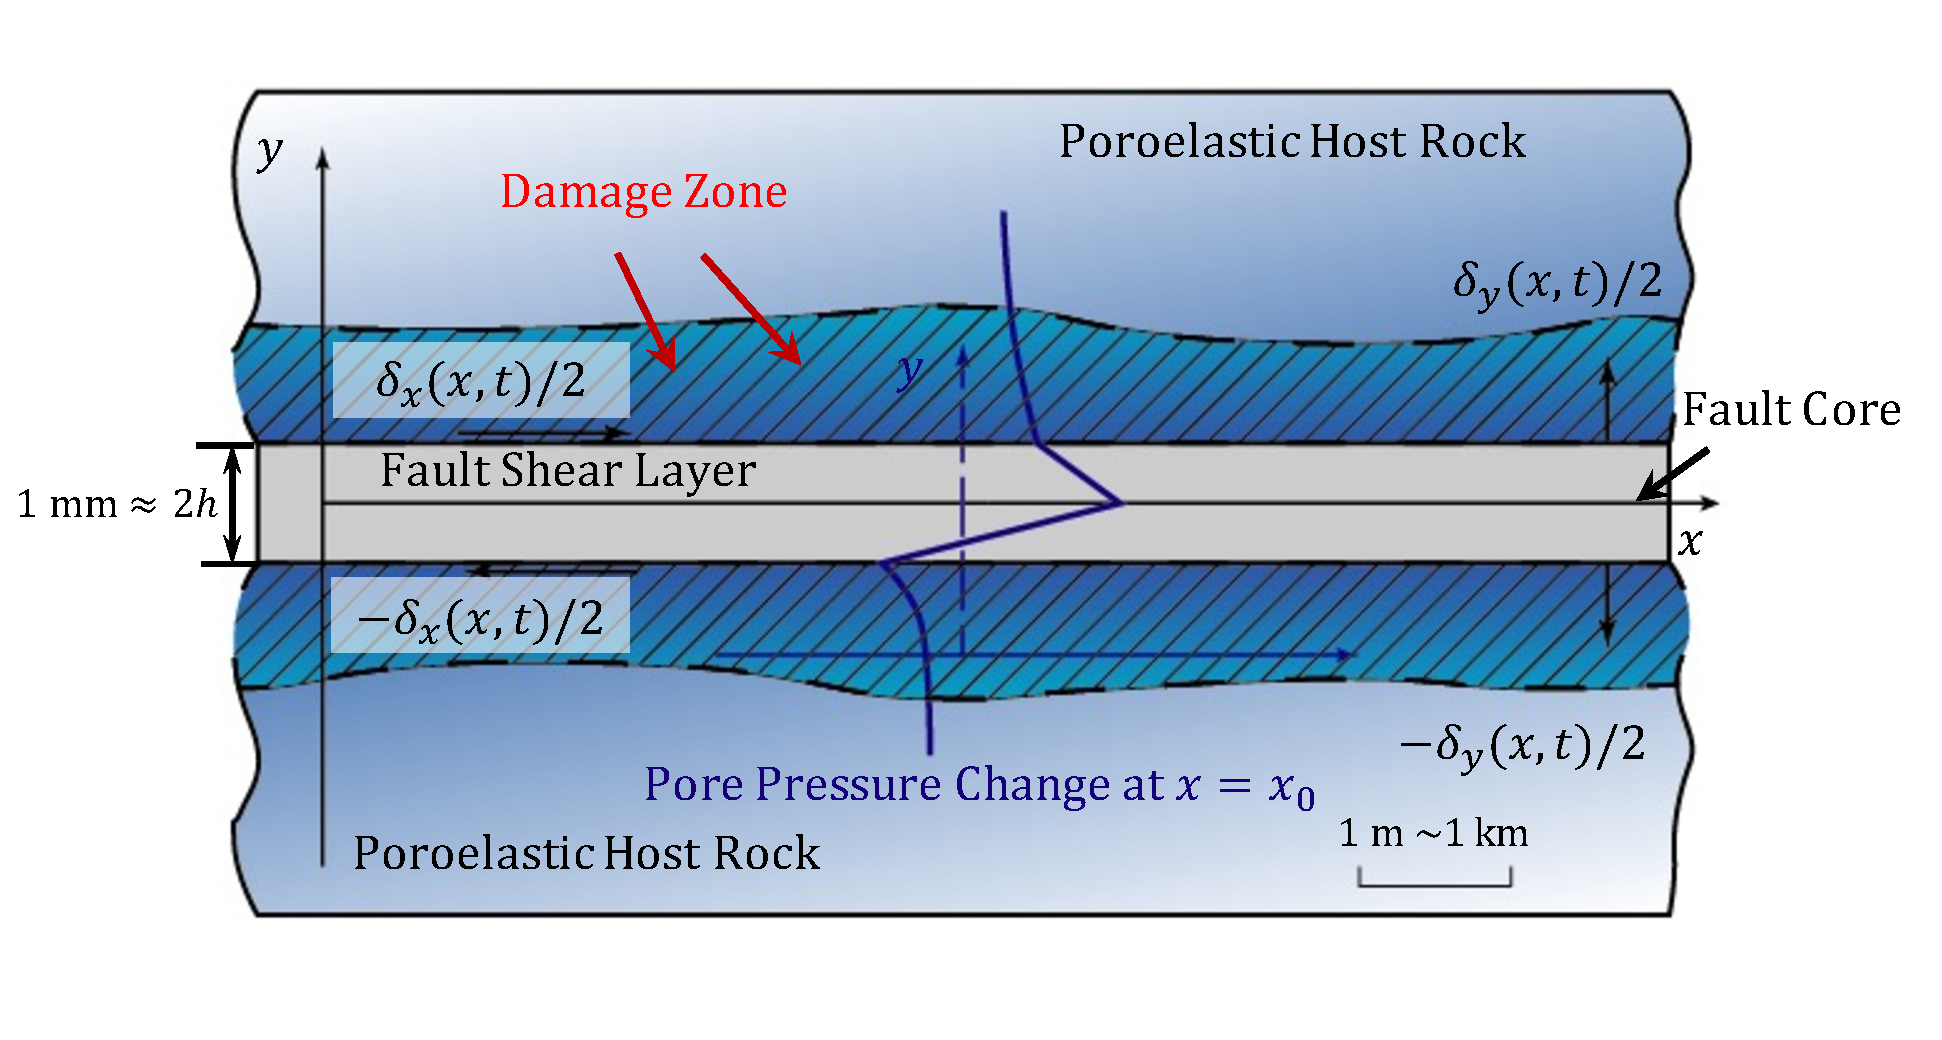
\includegraphics[width=1.0\textwidth]{final4.pdf}
    \caption{Model of pre-existing fault with poroelasticity, dilatancy, and damage zone.}
    \label{fig:conclusion 1}
\end{figure}

For example, Larochelle et al (2021) \cite{Larochelle_2021} studied fault slip under fluid injection using such a model supplemented with the along-interface fluid diffusion within the fault shear layer with a constant diffusivity.  The goal was to reproduce the results of a unique field experiment (Guglielmi et al., 2015 \cite{guglielmi_seismicity_2015}) and to examine the previously published conclusion (Bhattacharya et al., 2019 \cite{bhattacharya_induced_2019}) that the experimental data can only be explained by a model in which slow slip outruns the section of the fault pressurized by fluids.  
The study showed that a range of fault models can reproduce the outcomes of the field experiment, and the ones with higher reference friction (supported by laboratory studies) have slow slip well confined within the pressurized fault region, with important implications for fault stability and induced seismicity.   
While an advance over some previous studies of slip along pre-existing faults due to fluid injection, the modeling like in Larochelle et al. (2021) \cite{Larochelle_2021} is still significantly simplified. 

% Our goal is to build numerical models of sliding on pre-existing faults that more fully couple effects of fluids and nonlinear frictional fault slip, and validate those models through comparison with unique field and lab experiments. The important additional factors we would like to include are fluid pressure evolution due to inelastic shear dilatancy/compaction of the shearing layer, poroelasticity of the rock media, and changing poroelastic properties due to evolving off-fault damage (Figure~\ref{fig:future 2}). Inelastic dilatancy changes porosity, causing shear-induced evolution in pore fluid pressure within the layer; in part,  it can stabilize the fault slip acceleration by reducing the fault zone pore pressure \cite{segall_dilatancy_1995, Segall2010}. Poroelasticity causes changes in pore fluid pressure around the propagating shear rupture tip, since shear ruptures induce additional compressional and dilatational fields on the two sides of the fault, acting like a bi-material effect and inducing fluid flow across the shear layer and changes in the effective normal stress for the layer.  In part, these effects can destabilize fault slip in frictionally stable faults \cite{Heimisson2019}.  Off-fault damage changes permeability of the rock media \cite{faulkner_stuck_2011},with increases during slip events and healing in the inter-event period, as well as affects elastic properties and hence wave propagation \cite{Hudson1981}.  

While there are several numerical approaches for simulations of fluid flow in bulk rocks (e.g., Hart and Detournay, 1999 \cite{detournay_flac_1999}; Beljadid et al. \cite{Beljadid2020}, 2020; Cueto-Felgueroso et al., 2020 \cite{CuetoFelgueroso2020}), they typically do not include slip on well-developed pre-existing faults that can occur both quasi-statically and dynamically (with inertial effects, as during earthquakes). Developing such coupled numerical approaches is the goal of this work. The developed numerical approaches will be used to model field and lab experiments (e.g. Guglielmi et al., 2015 \cite{guglielmi_seismicity_2015}) as well as applied to induced seismicity and tectonic earthquakes. 
\section{Method}
\label{sec:method}
In this study, 
we essentially follow Heimisson et al. \cite{Elias_2021, Elias_Shengduo_2022} for theoretical and numerical modeling of dynamic fault slip.
\subsection{Governing equations}
The governing equations for the poroelastic solid bulk are
\begin{align}
    Gu_{i,kk}+\frac{G}{1-2\nu}u_{k,ki}&=\alpha p_{,i} \label{eq:poro1}\\
    \frac{1}{M}p_{,t}-\kappa p_{,kk}&=-\alpha u_{k,kt} \label{eq:poro2}, 
\end{align}
where $G$ and $\nu$ are elastic shear modulus and Poisson's ratio in drained condition.
$M$ and $\alpha$ are poroelastic Biot modulus and Biot coefficient, 
respectively.
$\kappa$ is the mobility of fluid in porous medium. 
The apparent fluid diffusivity from (\ref{eq:poro2}) is $c = M \kappa$. 
However, 
since $u$ on the right hand side of (\ref{eq:poro2}) is coupled with $p$, 
the apparent $c$ does not directly reflect the diffusion of fluid content. 
Through a change of variable, 
the actual fluid diffusion for the fluid mass content $\zeta$ is given by \cite{Rice_1998_notes}
\begin{align}
    \zeta_{,t} - c_{mass} \zeta_{, kk} = 0 \label{eq:massDiffusion}, 
\end{align}
where $c_{mass}$ is given by 
\begin{align}
    c_{mass} = c \frac{K_d+\frac{4}{3} G}{K_u + \frac{4}{3} G} \label{eq:cmass}. 
\end{align}
In (\ref{eq:cmass}), 
$K_d$ and $K_u$ are drained and undrained bulk modulus, 
respectively. 
In addition to poroelastic bulk, 
in this study, 
we consider elastic but permeable bulk to further compare the poroelastic effects with solely bulk fluid diffusion.
The governing equations for elastic permeable bulk are 
\begin{align}
    Gu_{i,kk}+\frac{G}{1-2\nu}u_{k,ki}&=0 \label{eq:elastic1}\\
    p_{,t} - c p_{,kk}&= 0\label{eq:elastic2}, 
\end{align}
where $c$ is the bulk diffusivity associated with the elastic permeable bulk. 
Note that for elastic permeable solid, 
since (\ref{eq:elastic2}) is independent of $u$, 
the apparent diffusivity coincides with the mass diffusivity, i.e., 
$c_{mass} = c$. 

\subsubsection{Frictional shear layer}
Then for the shear layer, 
rate and state friction model is given by (\ref{eq:RSF1}, \ref{eq:RSF2}). 
By setting $\dot{\theta} = 0$, 
one can obtain the steady-state friction relation as
\begin{align}
    \theta_{ss} &= \frac{D_{RS}}{V} \label{eq:thetaSS} \\
    \tau_{ss}(V) &= \sigma_{eff}\left[f_* + (a-b)\log\left(\frac{V}{V_*}\right) \right] \label{eq:RSss}, 
\end{align}
and the fault is considered rate-strengthening, 
if $a-b>0$ because steady state friction increases with slip rate. 
Similarly,
the fault is considered rate-weakening if $a-b<0$.
There is a minimum slip zone size for dynamic events to nucleate \cite{ruina_slip_1983}. 
\begin{align}
    L_{slip}\ge L_{nu} \propto \frac{GD_{RS}}{(b-a)(\sigma_n-p)} \label{eq:Lnu}.
\end{align}

Besides friction,
fluid mass transport within the shear layer as well as between the shear layer and the bulk also affects the slip. 
Figure~\ref{fig:poroshear1} lists the variables involved in this problem, 
where $\delta_p^+, \delta_p^-, \delta p_c$ are the fluid pore pressure change above, 
below and in the middle of the layer, 
respectively. 
$\delta_x, \delta_y$ are fault slip and opening, 
$\kappa, \kappa_{cx}, \kappa_{cy}$ are fluid mobilities in the bulk, 
in $x$ direction of the layer, 
in $y$ direction of the layer, 
respectively. 
Based on the modeling of (Elias et al., 2022) \cite{Elias_Shengduo_2022}, 
one can get the governing equation of $\delta p_m, \sigma$ and $\theta$ as following:
\begin{align}
    \delta p_m + \frac{\beta_f^\sigma - \beta_\phi^\sigma}{\beta_f^p+\beta^p_\phi}\sigma = \frac{1}{\phi_*(\beta_f^p+\beta^p_\phi)}\left(
    \frac{Q(X,t)}{\rho_{f*}}-\phi^{pl}+\int_0^t\frac{\kappa_{cy}}{h^2}\left(\frac{1}{2}(\delta p^+ + \delta p^-)- \delta p_c\right)+\kappa_{cx}\frac{\partial^2 \delta p_m}{\partial x^2} dt'
    \right) \label{eq:layerControl1}, 
\end{align}
where $\delta p_m =\frac{1}{2}\left(\frac{1}{2}(\delta p^++ \delta p^-)+\delta p_c\right)$
is the average pore pressure change within the fault shear layer, 
through piecewise linear approximation.
$\phi_*, \rho_{f*}$ are constants of reference porosity and fluid mass density.
$Q(X, t)$ is the total amount of injected fluid mass at $(X, t)$. 
$\phi^{pl}$ is shear layer dilatancy. 
$\beta$s are constant material compressibilities. 

\begin{figure}[hbtp]
    \centering
    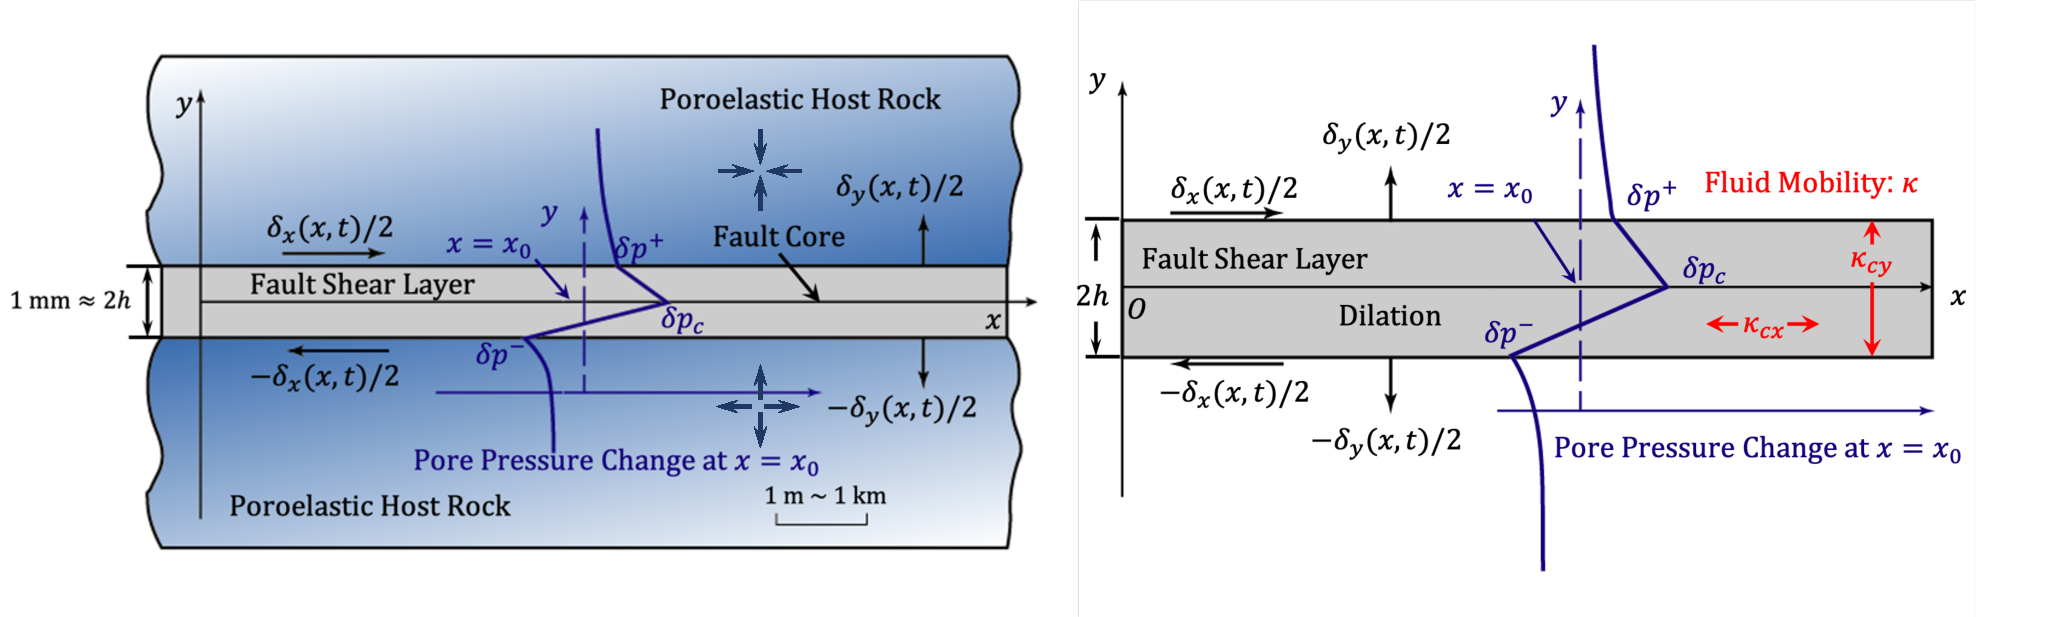
\includegraphics[width=1.0\textwidth]{poroelastic_layer1.pdf}
    \caption{Fault embedded in poroelastic solid medium (left).
    A closer look at the shear layer discussed in the text, with $\delta p_c$ increasing from zero due to fluid injection (right).}
    \label{fig:poroshear1}
\end{figure}

Similarly from the mass conservation of solids in the fault shear layer, 
one can get the control equation on fault opening $\delta_y$ \cite{Elias_Shengduo_2022}.

\begin{align}
    \delta_y &= 2h \left(\frac{\phi_*}{1-\phi_*}\beta_\phi^p-\beta_s^p\right)
    \left(
    \delta p_m - \frac{\frac{\phi_*}{1-\phi_*}\beta_\phi^p+\beta_s^p}{\frac{\phi_*}{1-\phi_*}\beta_\phi^p-\beta_s^p}\sigma
    \right)+\frac{2h\phi^{pl}}{1-\phi_*}, 
    \label{eq:layerControl2}
\end{align}
where $\beta_\phi^p$ and $\beta_s^p$ are compressibility constants. 

Equation (\ref{eq:layerControl1}) and (\ref{eq:layerControl2}) together with Rate-and-State friction forms the control equations of the fault shear layer. 
Then by numerically solving the coupled poroelastic equations for the solid bulk and those control equations for the layer, 
one can study specific fault-slip problems with poroelastic and dilatancy effects.*

For the injector of fluid, 
since in this study we aim to study the effect of injection rate, 
injection-time profile, etc., 
we need a baseline case with the total mass of injected fluid controlled, 
based on which we modify the flux of injection vs. time and examine its effects on the fault slip. 
Motivated by the pressure-control injection in (Elias et al., 2022) \cite{Elias_Shengduo_2022}, 
we take their averaged flux over the experiment window (1400 s), 
and use that as our baseline flux. 
Figure~\ref{fig:FluxControl} shows the comparison between the evolution of pore fluid pressure and slip rate over the fault under pressure-control injection and flux-control injection with the same average flux. 
The material properties which are kept the same in both cases can be found in Table~\ref{tab:elasticBulk} and \ref{tab:fricPropsFault}. 
We find that the flux-control injection case has qualitatively similar response compared with the pressure-control injection, 
while the pore fluid pressures $p^+, p^-$ and $p_c$ increase faster with time upon the start of the injection. 
In the following discussion we will refer to the flux-control case with baseline flux $1\times10^{-4}\ \mathrm{Kg/(m\cdot s)}$ as the baseline case. 

\begin{figure}[htbp]
    \centering
    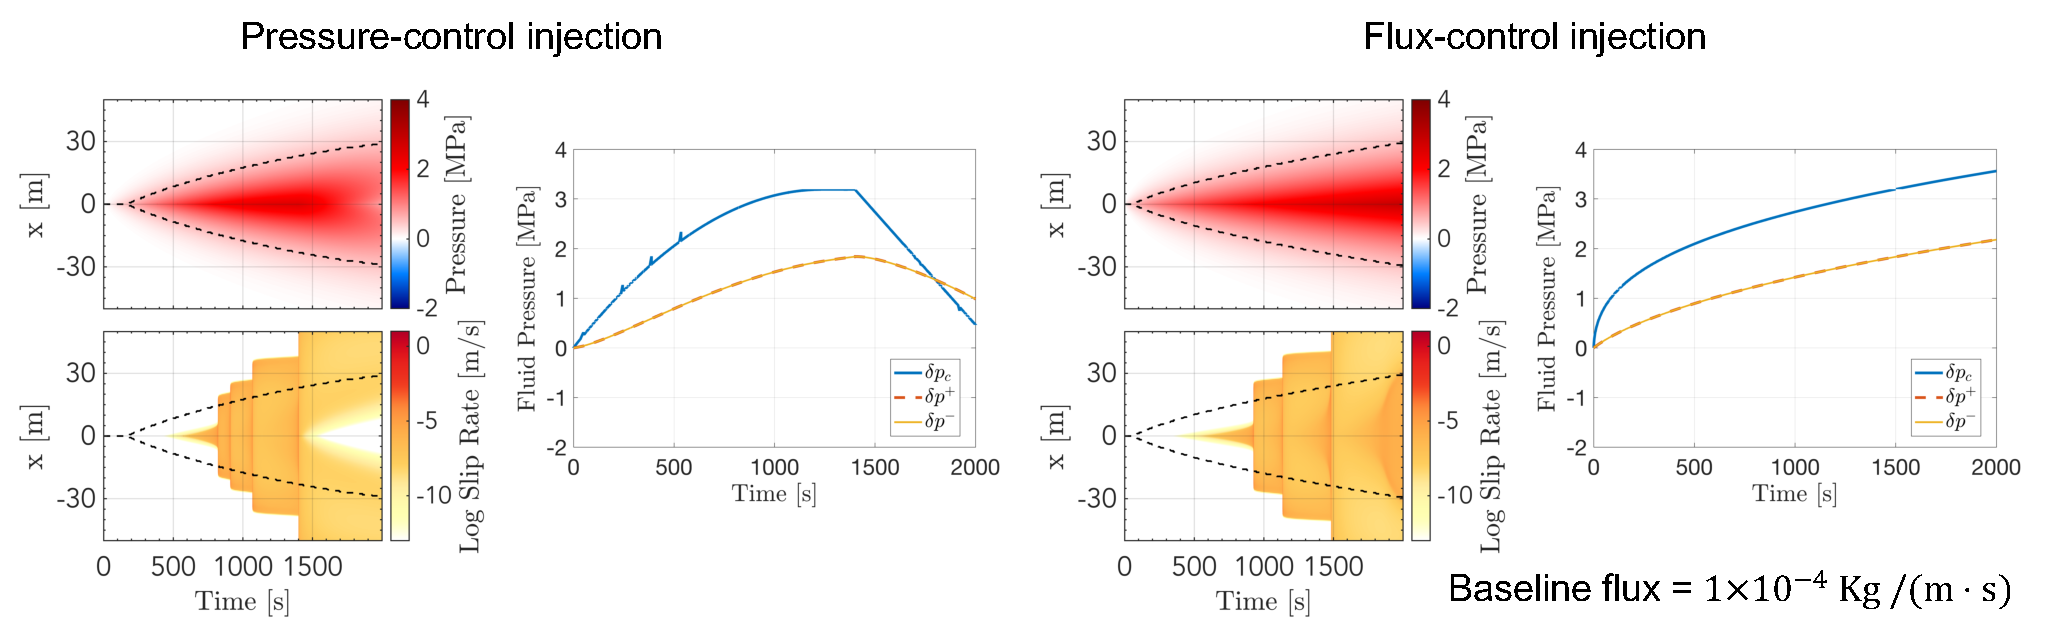
\includegraphics[width=1.0\textwidth]{figures/FluxControl.pdf}
    \caption{Comparison of slip rate and pore pressure evolution under pressure-control injection and flux-control injection. 
    The flux is set to be the average flux in the pressure-control injection case.}
    \label{fig:FluxControl}
\end{figure}
\section{Results and discussion}
\label{sec:resultsAndDiscussion}
In this section, 
we present and discuss results that reveal the effect of fault healing, 
poroelasticity, 
injection rate and more generally injection-time profile, 
on the stability of frictional fault slipping under fluid injection. 

\subsection{Fault healing affects the stability of fault slip significantly}
For a given loading traction of $\tau, \sigma$, 
friction coefficient is set to be $\tau / \sigma$. 
However, 
due to the competing effect of slip rate $V$ and the state variable $\theta$ in (\ref{eq:RSF1}), 
a more healed fault with larger $\theta$ will have a lower initial slip rate $V_{ini}$ under the same loading condition. 
Even though typical slip rate values over a fault long before the nucleation of dynamic events are close to $0$, 
we find that the initial healing (or slip rate) over the fault affects its dynamic behavior significantly under injection. 
Figure~\ref{fig:Vinitial} shows the comparison of slip and friction evolution for $V_{ini}\approx10^{-22}, 10^{-19}, 10^{-16}, 10^{-13}\ \mathrm{m/s}$ under the same flux-controlled injection. 
The flux-control injection in all the cases are kept the same as the baseline case, 
which has a flux of $10^{-4}\ \mathrm{Kg/(m\cdot s)}$ constant in time. 
Materials properties are listed in Table~\ref{tab:elasticBulk} and \ref{tab:fricPropsFault}. 
From figure~\ref{fig:Vinitial} (a) we see that as the fault gets less healed, 
which also means it has higher initial slip rate $V_{ini}$, 
the first dynamic event happens earlier in time, 
and also dynamic events happen more frequently. 
The events expand farther into the fault along $x$ direction. 
Figure~\ref{fig:Vinitial} (b) compares the slip rate at the center of the fault $x = 0$ for the above 4 cases. 
One can see that since the less-healed fault has higher $V_{ini}$, 
under the same injection flux it nucleates the first dynamic event earlier. 
Another thing to keep here is that once a dynamic event nucleates, 
the slip rate is of similar order of $10^{-1}\ \mathrm{m/s}$ for all cases. 
Figure~\ref{fig:Vinitial} (c) plots friction coefficient vs. slip for the above 4 cases. 
We see that the most-healed fault with $V_{ini}=10^{-22}\ \mathrm{m/s}$ has a friction peak of over $0.9$. 
The reason why more-healed faults lead to higher friction peak can be explained by the large gap between their lower initial slip rate and the dynamic slip rate of $0.1\ \mathrm{m/s}$. 
According to (\ref{eq:RSF2}), 
the evolution of $\theta$ happens at a scale of $D_{RS}$, 
and since there is hardly any slip happening before friction reaches its peak, 
$\theta$ is almost still at its initial value. 
Then by this approximation we can write 
\begin{align}
    f_{peak} - f_{ini} &= a \log\left(\frac{V_{dyn}}{V_{ini}}\right) \label{eq:deltF}, 
\end{align}
where $f_{peak}$, $f_{ini}=\tau / \sigma$ are the peak, initial friction; 
$V_{dyn}\approx 0.1\ \mathrm{m/s}$. 

In summary, 
we find that within the typical notion of ``close to zero" initial slip rate, 
the stability of fault slip under fluid injection depends significantly on the initial slip rate, 
and that less healed faults tend to have earlier, more frequent dynamic events that expand farther in space. 


\begin{figure}[htbp]
    \centering
    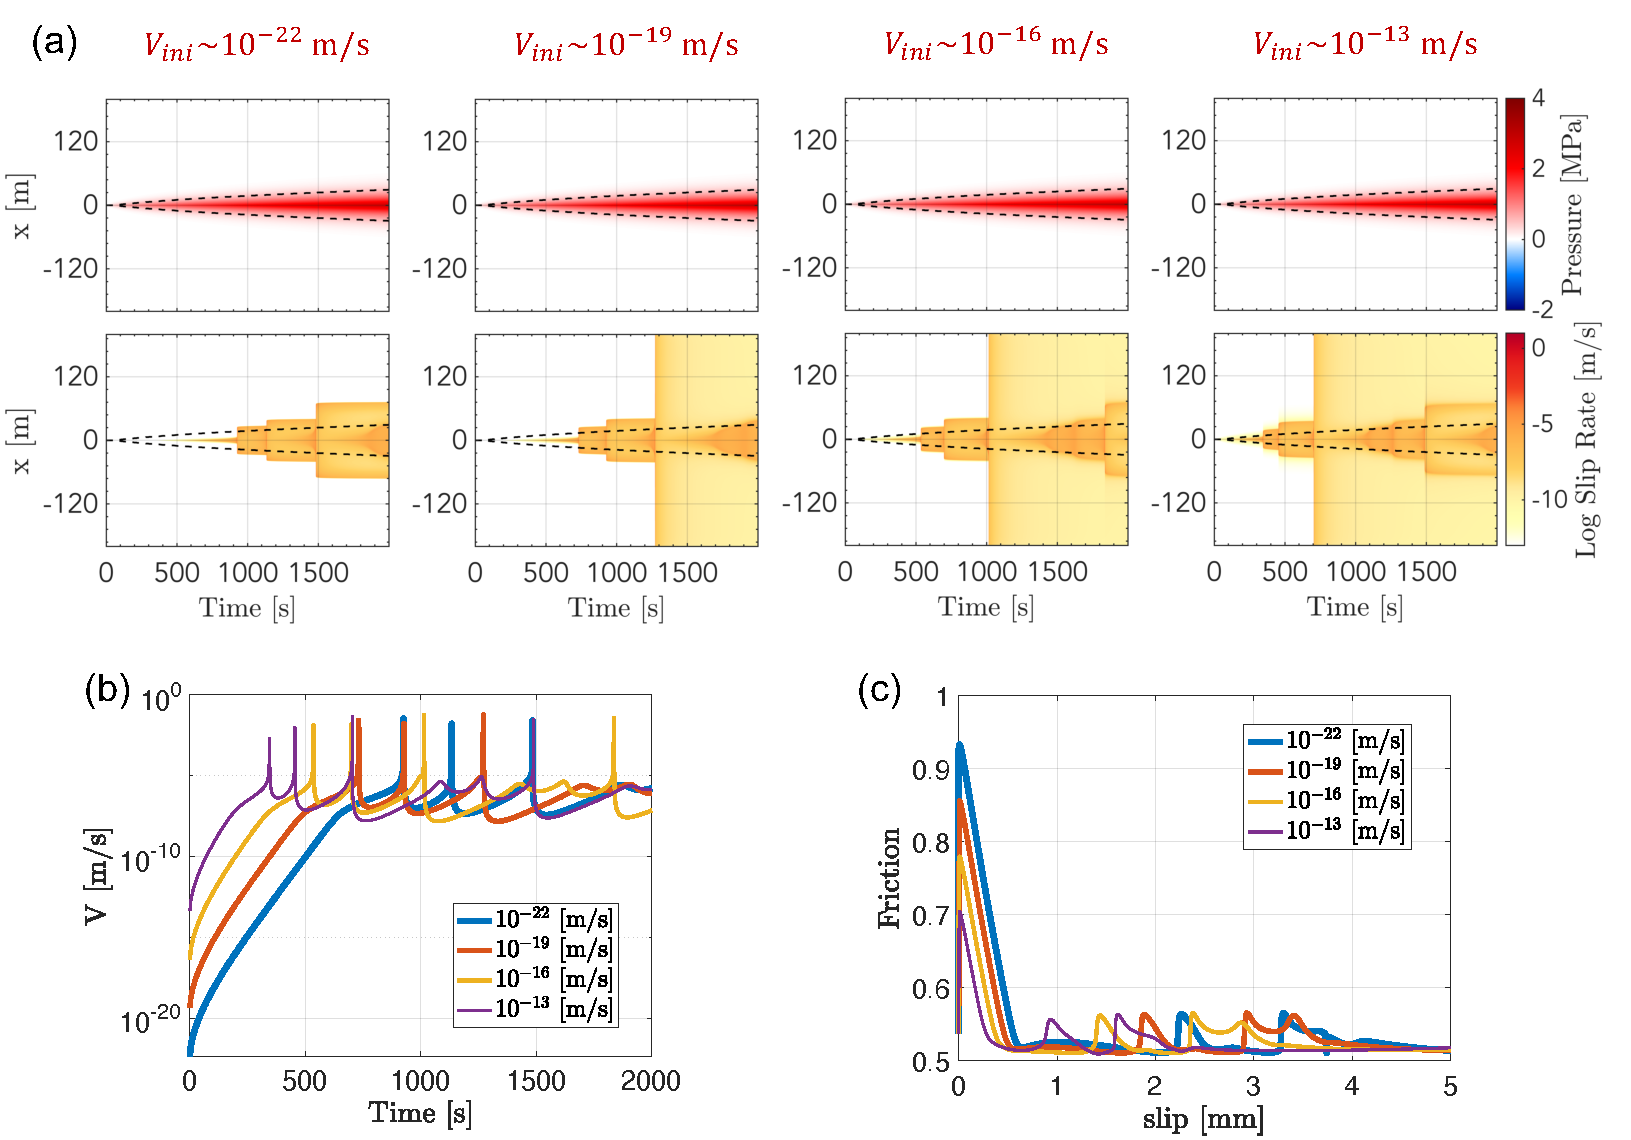
\includegraphics[width=1.0\textwidth]{figures/Vinitial.pdf}
    \caption{Less healed faults with higher initial slip rate tend to be more unstable under the same flux-controlled injection. (a) Comparison of pressure and slip rate vs. time along the fault for $V_{ini}\approx10^{-22}, 10^{-19}, 10^{-16}, 10^{-13}\ \mathrm{m/s}$. 
    (b) Slip rate vs. time at $x = 0\ \mathrm{m}$ for the above 4 cases. 
    (c) Friction vs. slip at $x = 0\ \mathrm{m}$ for the above 4 cases.}
    \label{fig:Vinitial}
\end{figure}

\subsection{Poroelastic effects stablize fault slip under injection}
In (Elias et al., 2022) \cite{Elias_Shengduo_2022}, 
researchers have shown that fault slip gets more unstable as the undrained Poisson's ratio $\nu_u$ decreases and gets closer to Poisson's ratio $\nu$, 
under the same fluid injection. 
And thus it was inferred that poroelasticicty stabilizes fault slip under fluid injection. 
However, 
due to the limitations in the code then, 
researchers were not able to achieve the elastic limit, i.e.,  $\nu_u = \nu$. 
In this study, 
we implement the elastic kernels such that we can indeed simulate cases with $\nu_u = \nu$, 
which equivalently sets $\alpha = 0$, 
and results in the poroelastic equations reduced to elastic equations as given by (\ref{eq:elastic1}, \ref{eq:elastic2}). 
To get a reasonable comparison between elastic and poroelastic cases, 
the governing equations and material properties of the shear layer are kept the same. 
The fluid mobility of the bulk $\kappa$ is kept the same between elastic and poroelastic cases, 
whereas the fluid diffusivity in the bulk is set to either $c=M\kappa$ or $c_{mass}$ given by (\ref{eq:cmass}). 

Since there are two relavant Poisson's ratios, 
namely the undrained $\nu_u$ and the drained $\nu$, 
we consider both elastic cases with Poisson's ratio set to $\nu_u$ and $\nu$, 
and compare them to the poroelastic case with $(\nu, \nu_u)$. 
The material properties are given in Tables~\ref{tab:elasticBulk} and \ref{tab:fricPropsFault}. 

\begin{figure}[htbp]
    \centering
    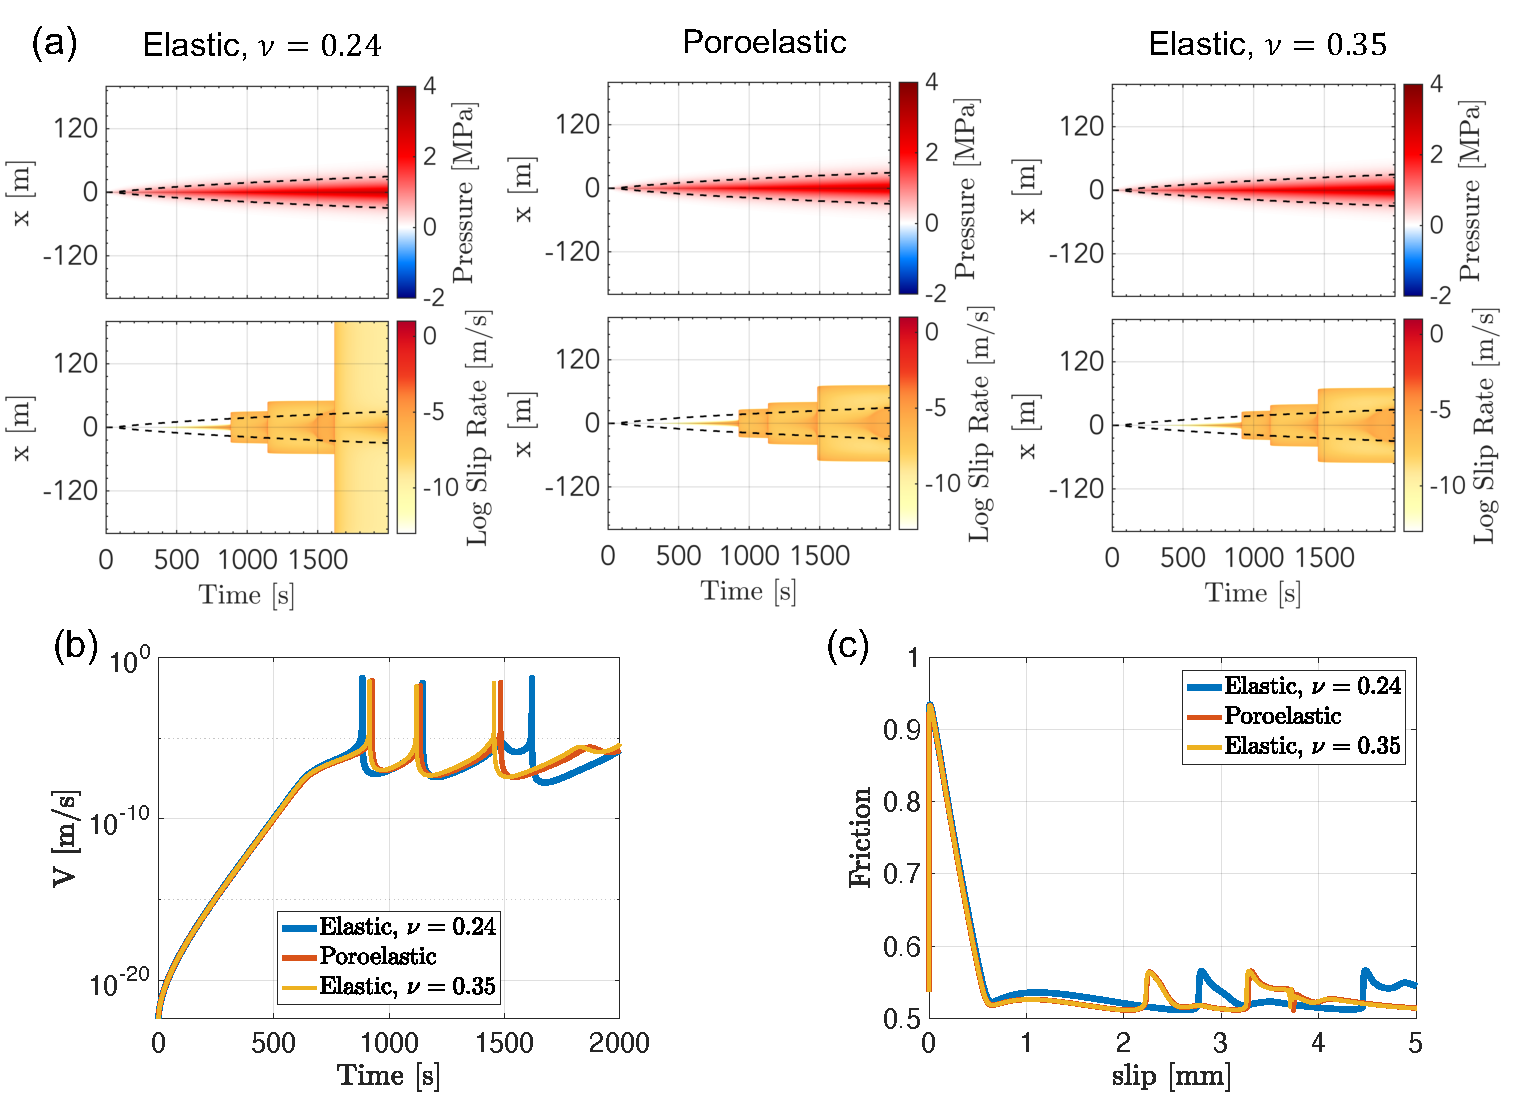
\includegraphics[width=1.0\textwidth]{figures/ElastPoro_c.pdf}
    \caption{Elastic, permeable vs. fully poroelastic bulk when the apparent bulk diffusivity $c$ is kept unchanged. (a) Comparison of average fluid pore pressure change $p_m$ and slip rate $V$ vs. time along the fault for elastic, $\nu = 0.24$, poroelastic ($\nu = 0.24, \nu_u = 0.35$), and elastic $\nu = 0.35$. 
    (b) Slip rate vs. time at $x = 0\ \mathrm{m}$ for the above 3 cases. 
    (c) Friction vs. slip at $x = 0\ \mathrm{m}$ for the above 3 cases.}
    \label{fig:ElastPoroC}
\end{figure}

\begin{figure}[htbp]
    \centering
    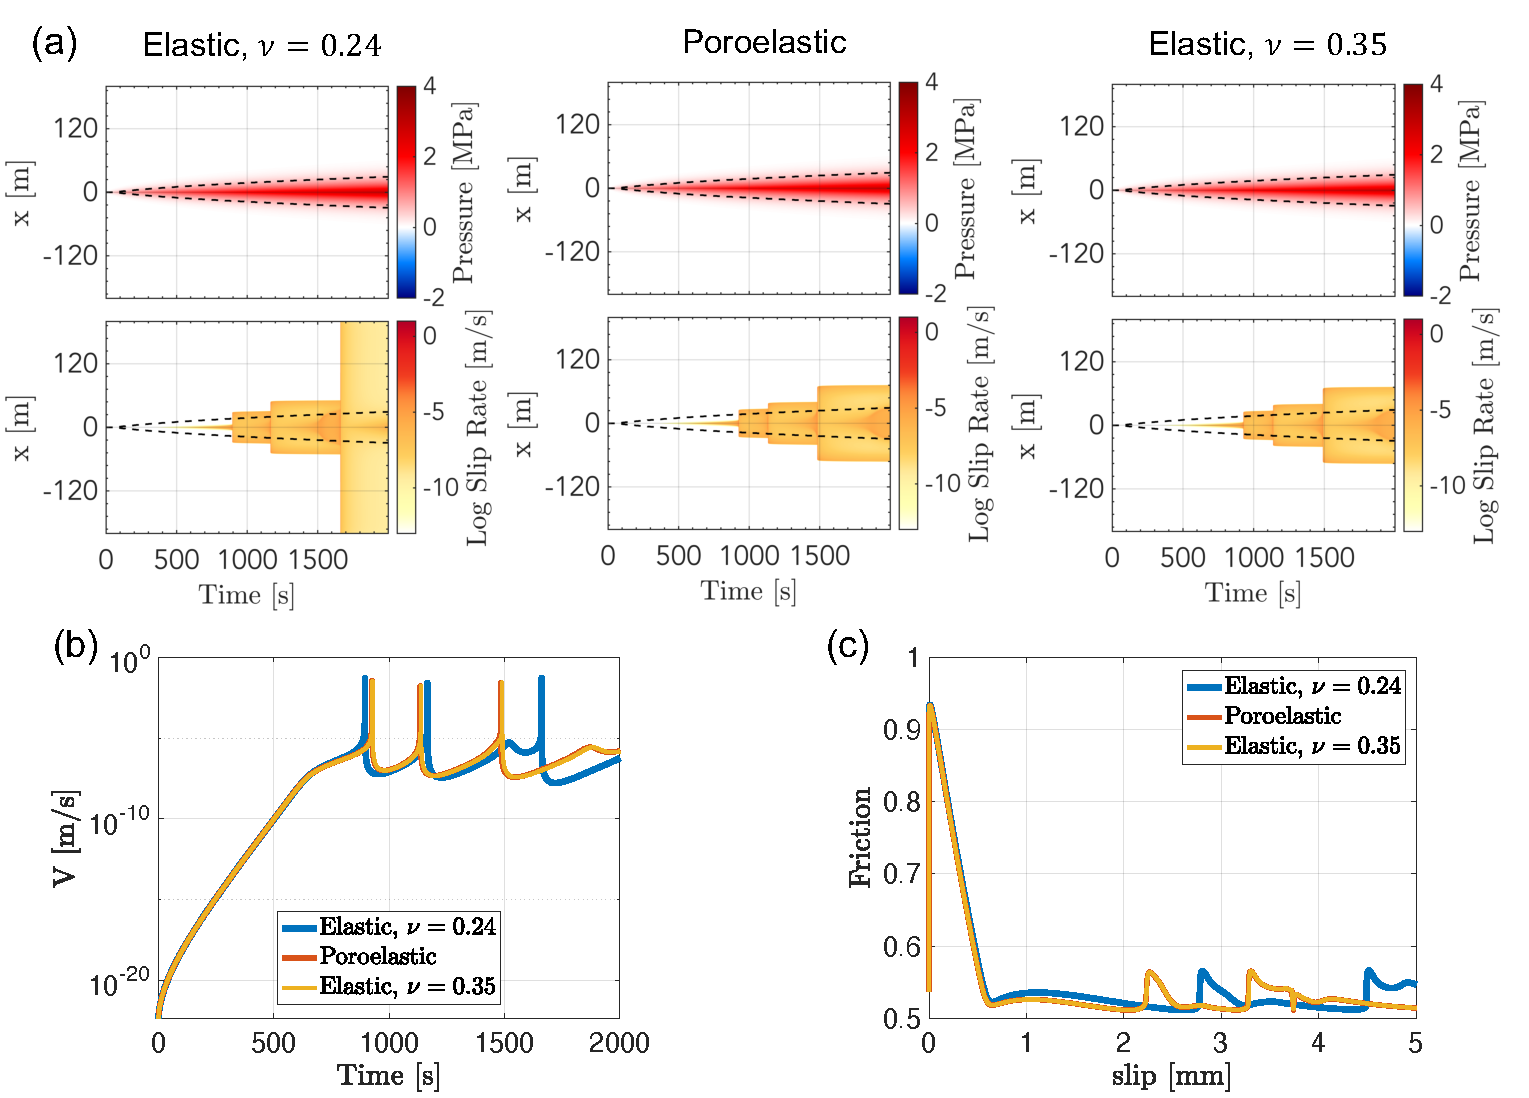
\includegraphics[width=1.0\textwidth]{figures/ElastPoro_cmass.pdf}
    \caption{Elastic, permeable vs. fully poroelastic bulk when the bulk diffusivity for fluid mass content $c_{mass}$ is kept unchanged. (a) Comparison of average fluid pore pressure change $p_m$ and slip rate $V$ vs. time along the fault for elastic, $\nu = 0.24$, poroelastic ($\nu = 0.24, \nu_u = 0.35$), and elastic $\nu = 0.35$. 
    (b) Slip rate vs. time at $x = 0\ \mathrm{m}$ for the above 3 cases. 
    (c) Friction vs. slip at $x = 0\ \mathrm{m}$ for the above 3 cases.}
    \label{fig:ElastPoroCMass}
\end{figure}

Figure~\ref{fig:ElastPoroC} and figure~\ref{fig:ElastPoroCMass} shows the comparison between elastic with drained Poisson's ratio (0.24), 
poroelastic, 
and elastic with undrained Poisson's ratio (0.35). 
The difference between the two figures is that cases in figure~\ref{fig:ElastPoroC} have the same apparent bulk diffusivity $c$, 
while cases in figure~\ref{fig:ElastPoroCMass} have the same $c_{mass}$ as given by (\ref{eq:cmass}). 
The middle columns in the two figures are from the same poroelastic case. 
Both figure~\ref{fig:ElastPoroC} and figure~\ref{fig:ElastPoroCMass} show that, 
under the same flux-control injection, 
the poroelastic case is much more stable than the elastic, permeable case with $\nu = 0.24$, 
and is slightly more stable than the elastic, 
permeable bulk with $\nu = 0.35$. 
This suggests that under such injection and dynamic fault slip condition, 
the poroelastic bulk is close to being undrained. 
Comparing the poroelastic case with elastic, $\nu = 0.35$ case in the two figures, 
we notice that if $c_{mass}$ is kept unchanged, 
using poroelastic bulk or elastic, permeable bulk have almost the same results, 
as shown by figure~\ref{fig:ElastPoroCMass}. 
The slip rate vs. time lines at $x = 0\ \mathrm{m}$ almost overlap perfectly for poroelastic and elastic, $\nu = 0.35$ bulk in figure~\ref{fig:ElastPoroCMass} (b), 
whereas in figure~\ref{fig:ElastPoroC} (b) those two corresponding lines are separating after $1000\ \mathrm{s}$. 
The conclusion is that one can get almost the same results of fault slip under such injection, 
if they replace poroelastic bulk with elastic, 
permeable bulk but keep $c_{mass}$, $\kappa$, $\nu_u$ and $G$ unchanged. 

A simple analysis shows that with realistic material properties of the bulk and the frictional interface, 
the poroelastic bulk would always be close to its undrained limit. 
Denote the characteristic length scale of the pressure front as $D_{ch}$, 
as shown in figure~\ref{fig:CloseTpUndrained}, 
which is usually a fraction of the fault length. 
Denote the propagation speed of the pressure front as $V_{pro}$, 
which is usually a fraction of the shear wave speed of the bulk. 
For any material point adjacent to the fault in the poroelastic bulk, 
the time it is affected by the pressure front is $t_{ch} = D_{ch} / V_{pro}$, 
in which time, 
by 1-D diffusion approximation, 
the pressure on the fault can expand $D_{sp} = \sqrt{t_{ch}c}$ into the bulk. 
For the fluid diffusion in the bulk to be prominent, 
in other words, 
for the bulk to be not almost undrained, 
we would need 
\begin{align}
    D_{sp} &= \sqrt{t_{ch} c_{req}} \approx D_{ch} \notag \\
    c_{req} &\approx D_{ch} V_{pro} \label{eq:estimateC}, 
\end{align}
where $c_{req}$ denotes the required fluid diffusivity, 
and is usually on the order of $10^{3}\ \mathrm{m^2/s}$, 
since $D_{ch}$ is at least on meter level, 
and $V_{pro}$ is on the order of $100\ \mathrm{m/s}$. 
Figure~\ref{fig:CloseTpUndrained} shows the propagation of the pressure front of a case with poroelastic bulk under baseline flux injection, 
in which case the required bulk diffusivity has to be $\approx 1200\ \mathrm{m^2/s}$ to be not almost undrained. 
\begin{figure}[htbp]
    \centering
    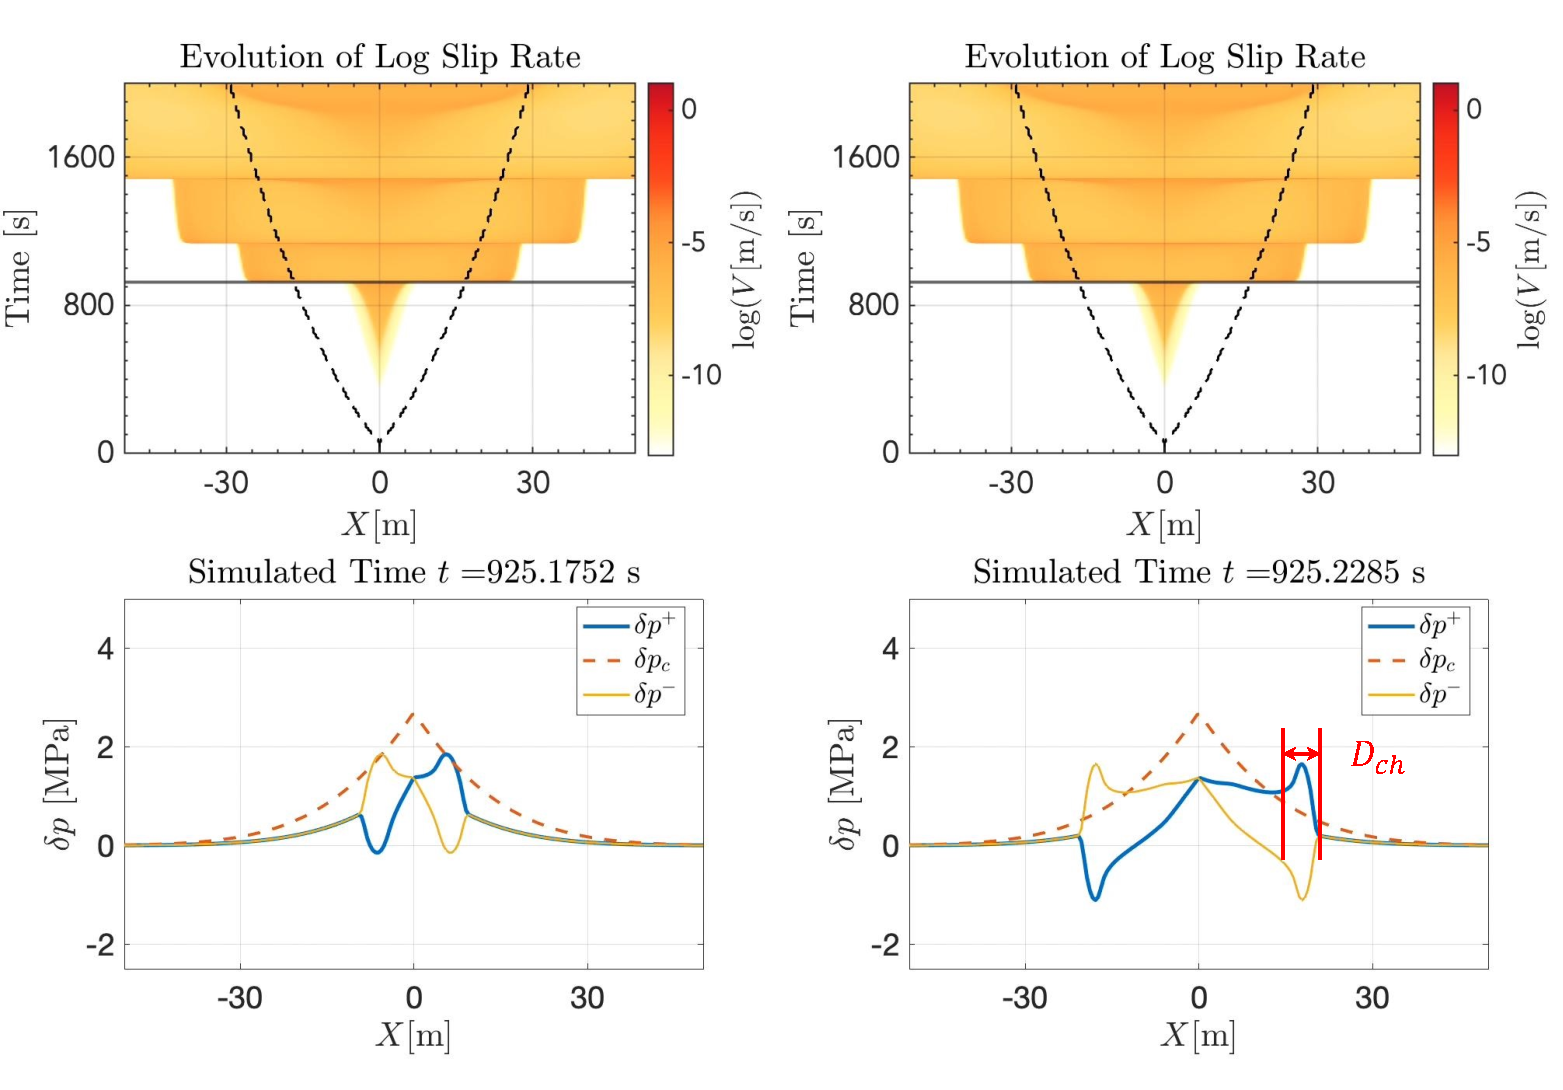
\includegraphics[width=1.0\textwidth]{figures/CloseToUndrained.pdf}
    \caption{The propagation of pressure separation during nucleation of dynamic events due to poroelastic effect. 
    The characteristic length scale of the perturbed pressure front is $D_{ch} \approx 6\ \mathrm{m}$, 
    and from the time difference of the two plots, 
    the propagation speed of the perturbed pressure feature is $V_{pro} \approx 200\ \mathrm{m/s}$
    }
    \label{fig:CloseTpUndrained}
\end{figure}

\subsection{Injection intermittently stabilizes fault slip compared to injection with constant flux} 
Besides studying the effect of poroelasticity vs. elasticity, 
we also look into how the injection flux affects the stability of fault slip. 
First we study for a fixed mass of fluid to be injected, 
whether changing the injection rate (flux) will lead to different fault slip. 
Figure~\ref{fig:fluxPoro} shows the comparison of slip rate vs. time along $x$ for an injection at baseline flux, 
0.75 baseline flux and 0.5 baseline flux. 
The surrounding bulk is poroelastic with properties listed in table~\ref{tab:elasticBulk}. 
The fault properties are listed in table~\ref{tab:fricPropsFault}. 
From figure~\ref{fig:fluxPoro} (a) we see that a larger injection rate leads to earlier, 
more frequent dynamic events but with smaller spatial extent. 
Especially with the smallest injection rate at 0.5 baseline flux, 
even if the dynamic event happens later and less frequently, 
it expands across the entire fault instantly. 
Figure~\ref{fig:fluxPoro} (b) suggests that the dynamic slip rate is similar for all injection rates once a dynamic event happens. 
(c) shows that the friction peak is similar among all three cases because they start from the same initial slip rate, 
and reached similar levels of dynamic slip rate. 

Figure~\ref{fig:fluxElas0.35} in the appendix shows qualitatively similar results for elastic, permeable bulk with undrained Poisson's ratio, 
which confirms that for a given total injected mass of fluid, 
larger injection rate would lead to more frequent but spatially more constrained dynamic slip events. 

\begin{figure}[htbp]
    \centering
    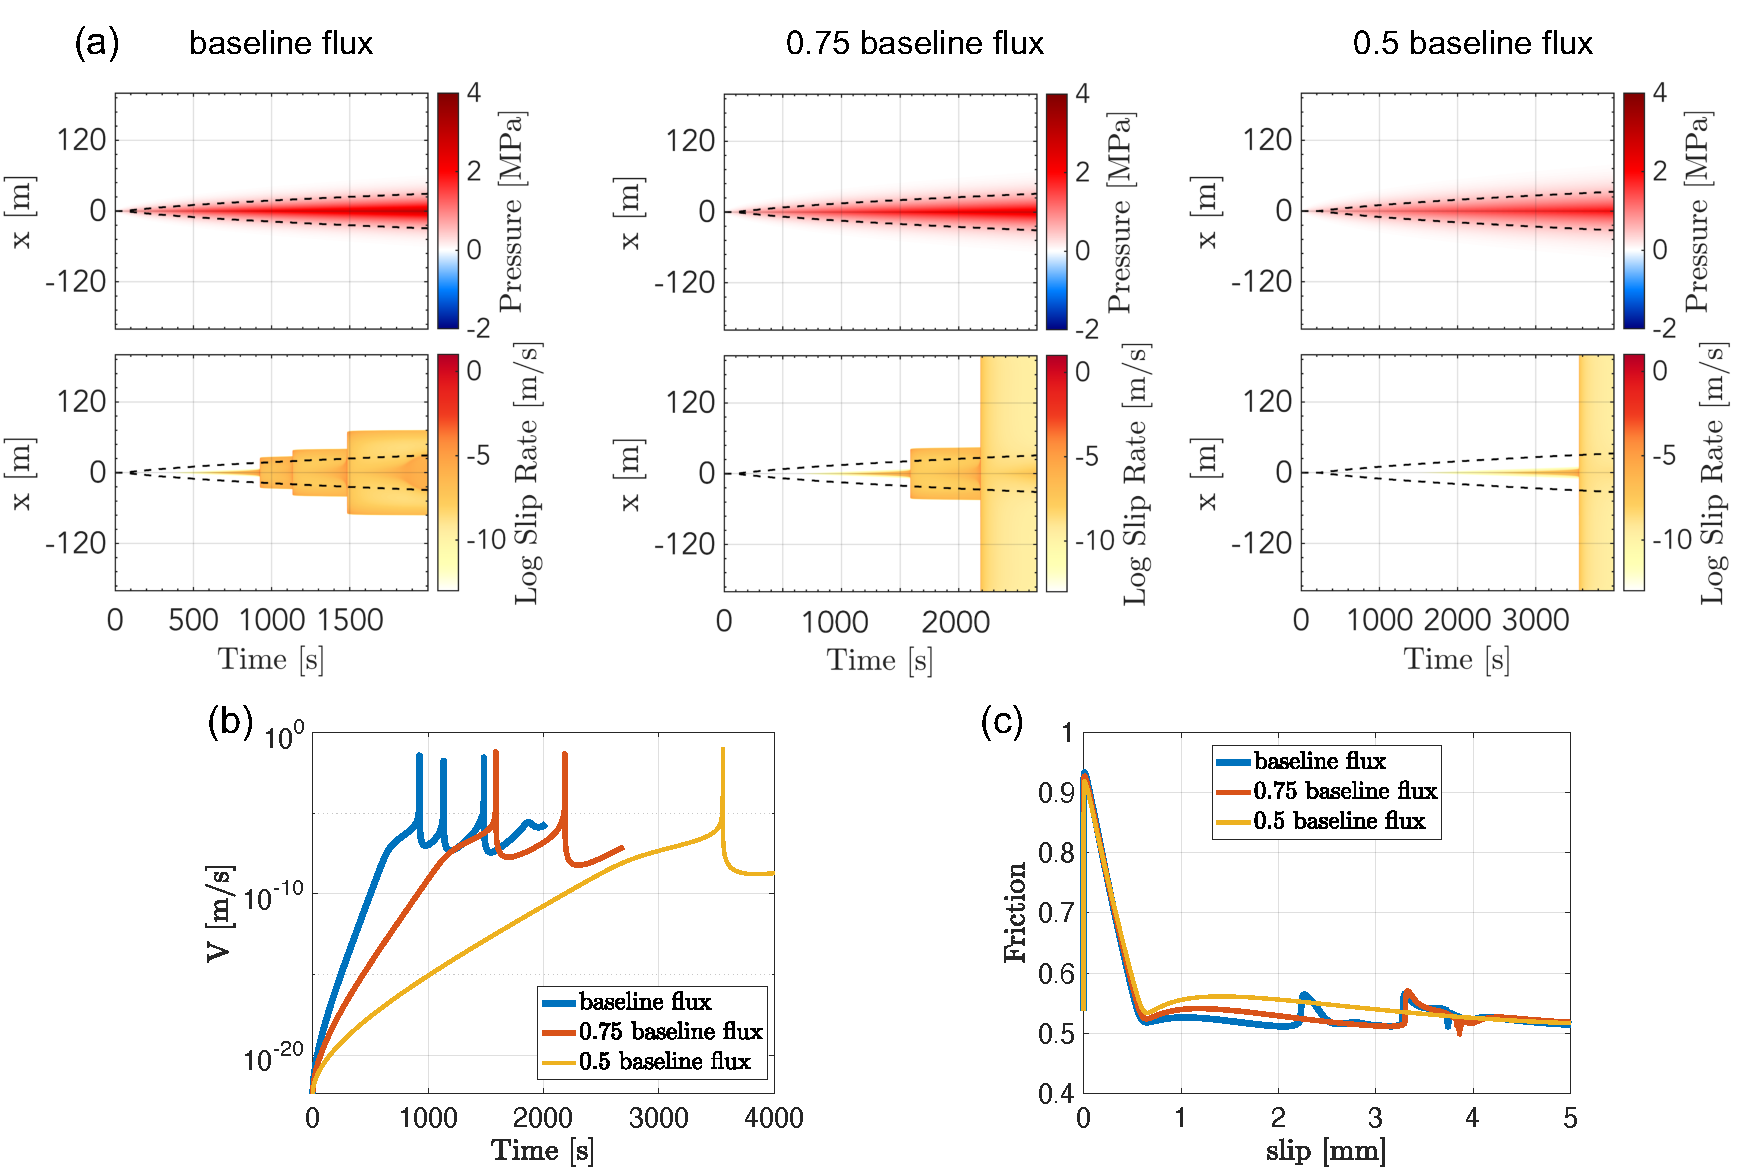
\includegraphics[width=1.0\textwidth]{figures/flux_poro.pdf}
    \caption{The effect of injection rate (flux) on stability of fault slip surrounded by poroelastic bulk. 
    The total injected mass is kept the same for all cases, 
    and thus time is adjusted for different injection rate. 
    Baseline flux is set to be $1.0\times10^{-4}\ \mathrm{Kg / (m \cdot s)}$.
    (a) Pore fluid pressure change and slip vs. time along $x$ for baseline flux, $0.75$ baseline flux and $0.5$ baseline flux. 
    (b) Slip rate vs. time at $x = 0\ \mathrm{m}$ for the above 3 cases. 
    (c) Friction vs. slip at $x = 0\ \mathrm{m}$ for the above 3 cases.}
    \label{fig:fluxPoro}
\end{figure}

Inspired by the fact that a faster injection rate delays the occurence of a spatially wide-spread dynamic event, 
which is usually more destructive, 
we change the injection rate from being constant to being intermittent in time, 
while at the same time also keep the average injection rate and total amount of injected mass the same. 
Figure~\ref{fig:constIntermittent} (b) shows the comparison of slip rate vs. time along the fault between constant and intermittent injection flux. 
The intermittent injection profile results in more frequent dynamic events, 
but none of them expand spatially to the entire fault. 
Figure~\ref{fig:constIntermittent} (c) confirms that in either case the dynamic events have a similar slip rate of $10^{-1}\ \mathrm{m/s}$. 
Since the dynamic events caused by intermittent injection have similar slip rate but more constrained spatial extent, 
it is usually less destructive. 
Figure~\ref{fig:constIntermittent} (d) further confirms that intermittent injection results in smaller total slip. 
This suggests that with some more carefully optimized injection rate-time profile, 
it is possible to achieve more spatially-restricted, 
less destructive dynamic slip events, 
with a given average injection flux as the constraint. 

\begin{figure}[htbp]
    \centering
    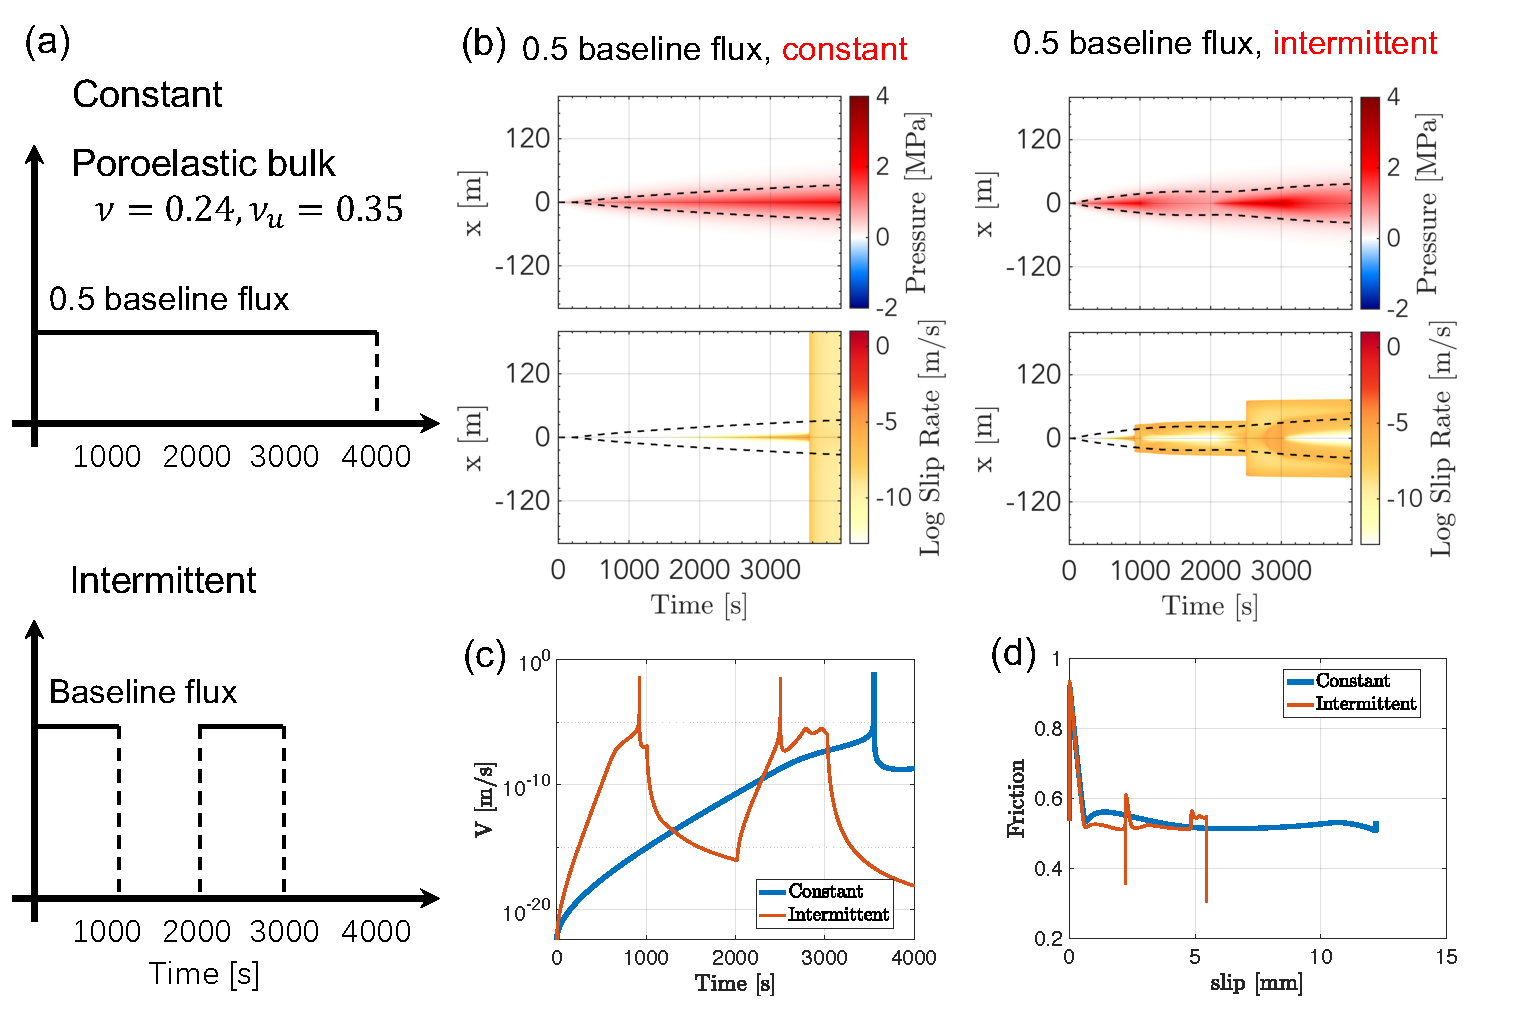
\includegraphics[width=1.0\textwidth]{figures/ConstIntermittent.pdf}
    \caption{Comparison between constant injection rate and intermittent injection rate with poroelastic bulk. 
    (a) Constant and intermittent injection rate as functions of intermittent. 
    (b) Pore fluid pressure change and slip rate vs. time along the fault for constant and intermittent injection rate.
    (c) Slip rate vs. time at $x = 0\ \mathrm{m}$. 
    (d) Friction coefficient vs. slip at $x = 0\ \mathrm{m}$.}
    \label{fig:constIntermittent}
\end{figure}
\section{Conclusions}
\label{sec:conclusions}
\ifincludetext{
In this study, 
we apply and further develop a boundary integral code for simulations of frictional fault slip, 
with poroelastic surrounding bulk, 
to study several relevant factors that may affect the stability of fault slip under fluid injection. 
First, 
we find that the fault healing, or initial slip rate under rate-and-state friction, 
affects the stability of fault slip significantly. 
A change from $V_{ini} = 10^{-22}\ \mathrm{m/s}$ to $V_{ini} = 10^{-13}\ \mathrm{m/s}$ would result in a much earlier nucleation of dynamic events and much larger spatial expansion of them, 
under the same fluid injection. 
Second, 
we further develop the code to allow for purely elastic bulk with the same fluid-transport properties, 
and confirm that poroelasticity stabilizes fault slip under fluid injection. 
We also find that with the typical length scales and properties of natural faults as well as injection time scale, 
poroelastic and elastic bulk with undrained Poisson's ratio have similar effects on dynamic fault slip. 
This is because the propagation speed of the pore pressure front is much faster than the diffusion speed of the pressure perturbations into the bulk, 
and thus the bulk s essentially undrained elastic. 
Finally, 
we study the effects of injection flux as a function of time on the stability of fault slip. 
We find that for mass-controlled injection at constant injection rate, 
higher injection rate leads to earlier and more frequent occurrences of dynamic events. However, these events have smaller spatial extent.
Motivated by that, 
we further change the injection rate from constant to intermittent in time, 
and find that with the same average injection rate and total injected fluid mass, 
intermittent injection also leads to earlier, 
more frequent but more spatially restricted dynamic events. 
This suggests that with an optimized injection rate-time profile, 
one can possibly achieve more spatially restricted and less destructive dynamic events at a given average injection rate. 
In the future, 
one can formulate an optimization over injection rate-time function, 
to achieve an objective of more stable, 
less destructive dynamic fault slip under a given average injection rate.
}
\fi
%% The Appendices part is started with the command \appendix;
%% appendix sections are then done as normal sections
\newpage
\appendix
\section{Values of material properties used in the simulations}\label{sec:Tables}
% The linear elastic properties of Homalite-100:
% Table~ for elastic properties of Homalite-100
\begin{table}[H]
    \centering
    \begin{tabular*}{0.8\textwidth}{ @{\extracolsep{\fill}} cccccc}
    \toprule
    $G\ [\mathrm{GPa}]$ & $\nu$ & $\alpha$ &  $M\ [\mathrm{GPa}]$ & $\kappa\ [\mathrm{m^2/(Pa\cdot s)}]$ & $c [\mathrm{m^2/s}]$\\
    \midrule
    $10$ & $0.24$ & $0.5530$ & $0.35$ & $2.1688\times10^{-19}$ & $1.0\times10^{-8}$ \\
    \bottomrule
    \end{tabular*}
    \caption{Linear poroelastic material properties of the bulk material}
    \label{tab:elasticBulk}
\end{table}

% Rate-and-state friction properties of Homalite-100 interfaces:
% Table~ for rate-and-state properties
\begin{table}[H]
    \centering
    \begin{tabular*}{0.9\textwidth}{ @{\extracolsep{\fill}} ccccccc}
    \toprule
    $f_*$ & $V_*\ [\mathrm{m/s}]$ & $a$ & $b$ & $D_{RS}\ [\mathrm{m}]$ & $\kappa_{cx}\ [\mathrm{m^2/(Pa\cdot s)}]$ & $\kappa_{cy}\ [\mathrm{m^2/(Pa\cdot s)}]$\\
    \midrule
    $0.55$ & $1.0\times 10^{-6}$ & $0.0112$ & $0.0160$ & $16.75\times 10^{-6}$ & 8.75834 \times 10^{-11} & 8.75834 \times 10^{-20}\\
    \bottomrule
    \end{tabular*}
    \caption{Friction and diffusivity properties of the fault interface}
    \label{tab:fricPropsFault}
\end{table}

\section{Supplementary figures}
\begin{figure}[htbp]
    \centering
    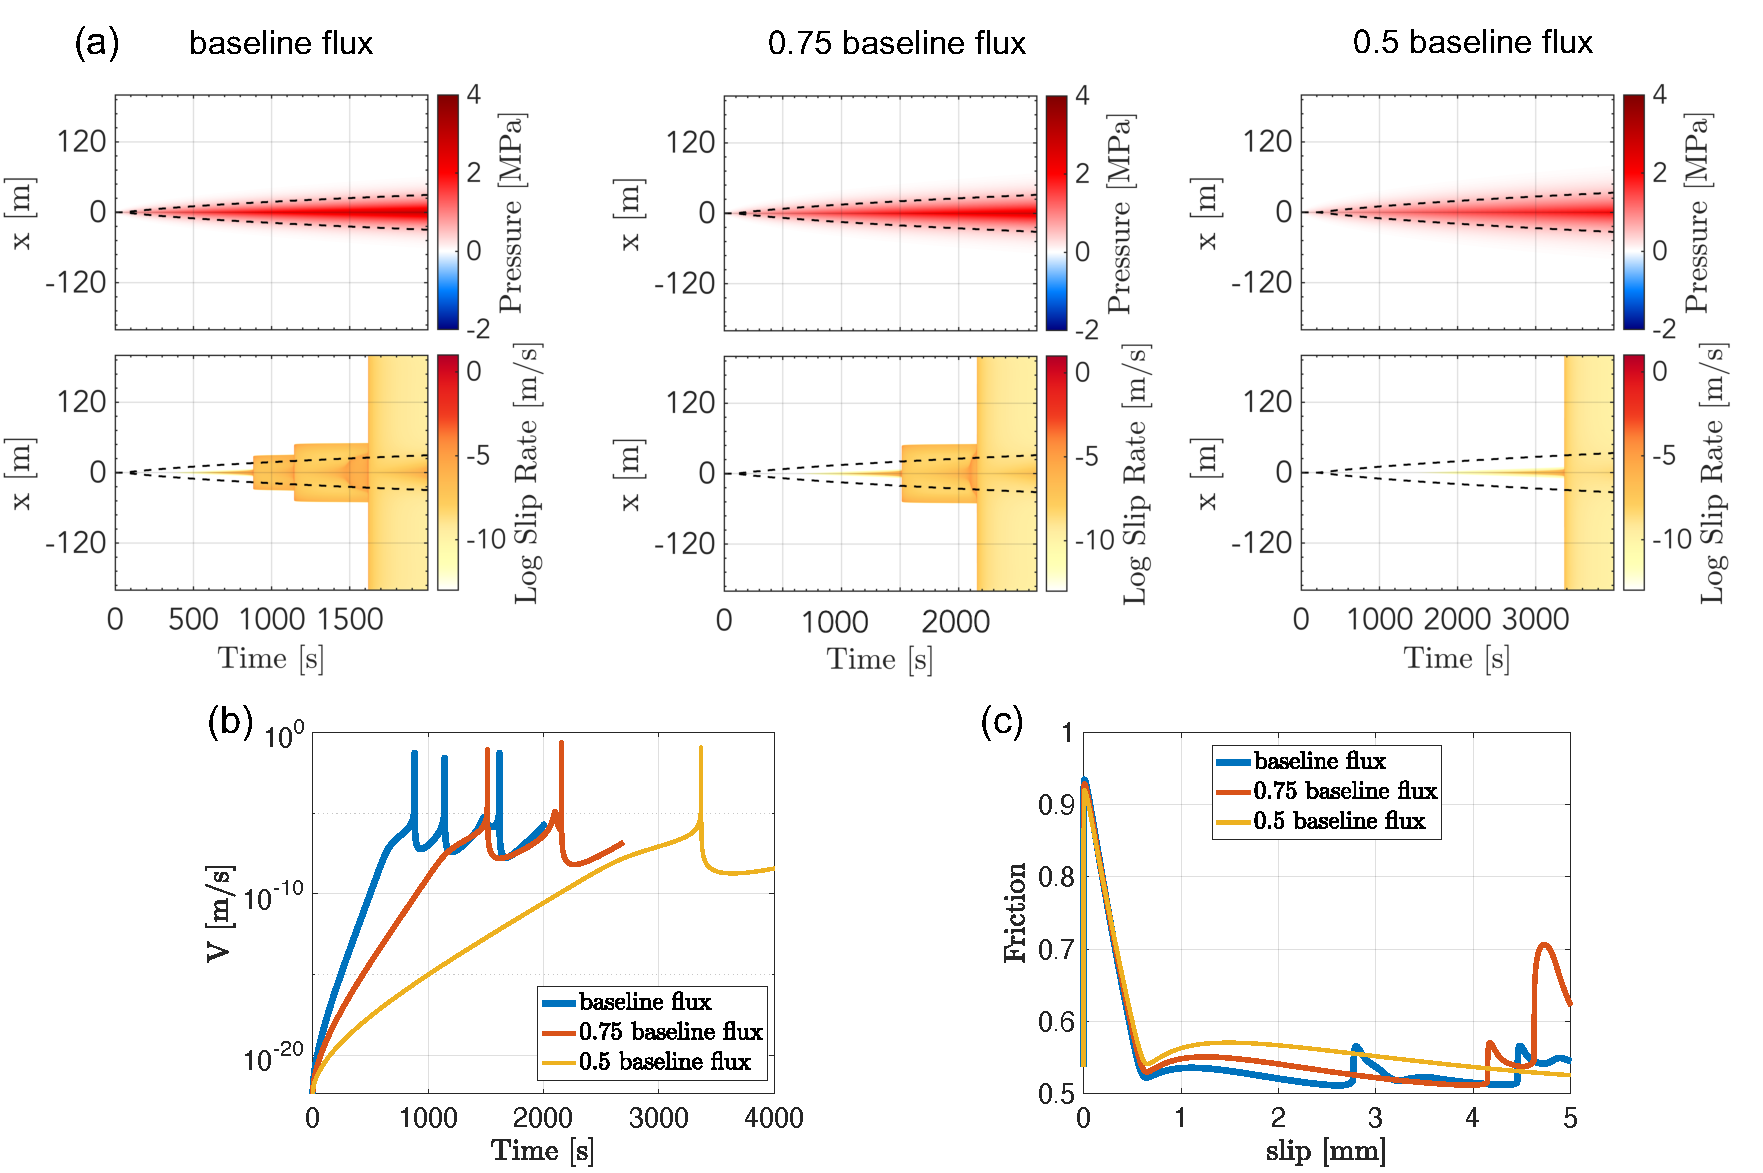
\includegraphics[width=1.0\textwidth]{figures/flux_elast_0.24.pdf}
    \caption{The effect of injection rate (flux) on stability of fault slip surrounded by elastic, permeable bulk with $\nu = 0.24$. 
    The total injected mass is kept the same for all cases, 
    and thus time is adjusted for different injection rate. 
    Baseline flux is set to be $1.0\times10^{-4}\ \mathrm{Kg / (m \cdot s)}$.
    (a) Pore fluid pressure change and slip vs. time along $x$ for baseline flux, $0.75$ baseline flux and $0.5$ baseline flux. 
    (b) Slip rate vs. time at $x = 0\ \mathrm{m}$ for the above 3 cases. 
    (c) Friction vs. slip at $x = 0\ \mathrm{m}$ for the above 3 cases.}
    \label{fig:fluxElas0.24}
\end{figure}

\begin{figure}[htbp]
    \centering
    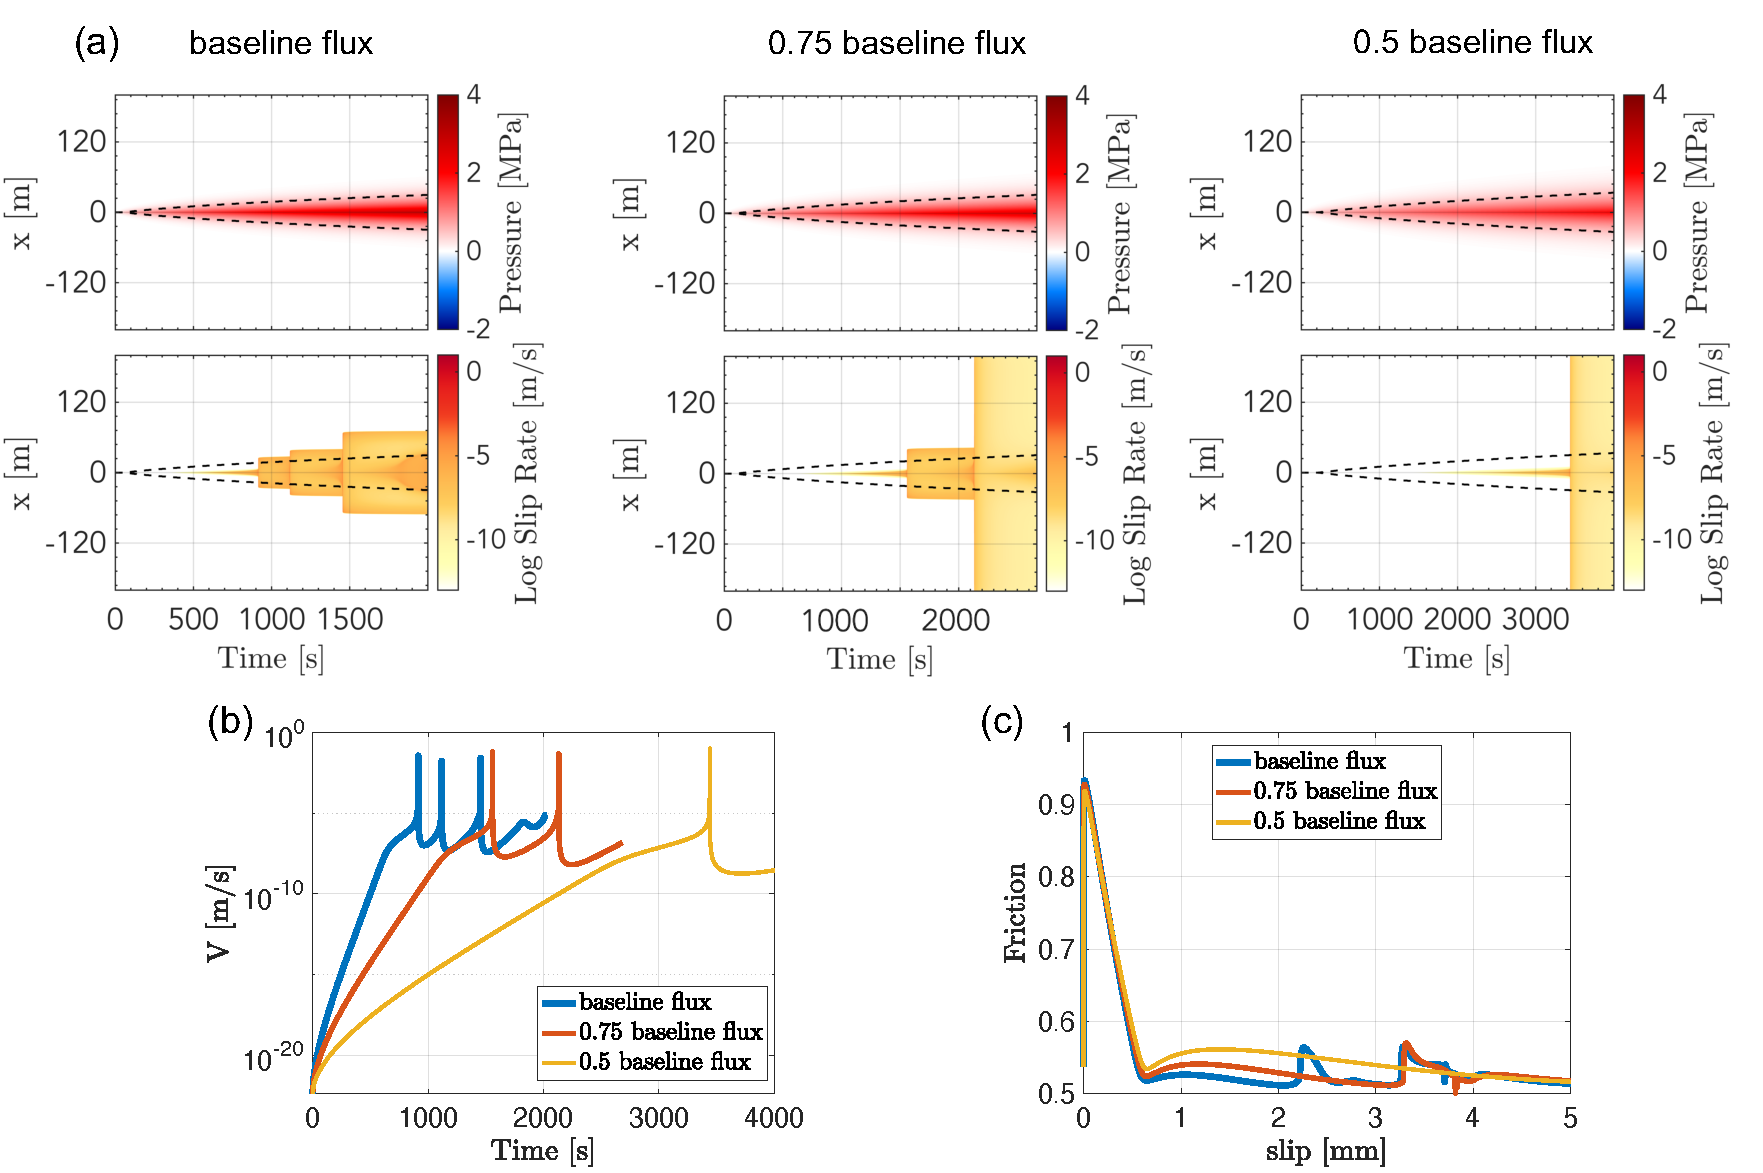
\includegraphics[width=1.0\textwidth]{figures/flux_elast_0.35.pdf}
    \caption{The effect of injection rate (flux) on stability of fault slip surrounded by elastic, permeable bulk with $\nu = 0.35$. 
    The total injected mass is kept the same for all cases, 
    and thus time is adjusted for different injection rate. 
    Baseline flux is set to be $1.0\times10^{-4}\ \mathrm{Kg / (m \cdot s)}$.
    (a) Pore fluid pressure change and slip vs. time along $x$ for baseline flux, $0.75$ baseline flux and $0.5$ baseline flux. 
    (b) Slip rate vs. time at $x = 0\ \mathrm{m}$ for the above 3 cases. 
    (c) Friction vs. slip at $x = 0\ \mathrm{m}$ for the above 3 cases.}
    \label{fig:fluxElas0.35}
\end{figure}


%% If you have bibdatabase file and want bibtex to generate the
%% bibitems, please use
%%
\newpage
 \bibliographystyle{elsarticle-num} 
 \bibliography{cas-refs}

\end{document}
